%__________________________________________________________________________________

\chapter{Local-Timed Negotiations}
\label{chap:ltn}

Chapter~\ref{chap:preliminaries} recalled \emph{negotiations} as an
interaction-centric model of concurrency, and \emph{timed automata} as a standard
framework for real-time constraints.  This chapter introduces
\emph{local-timed negotiations} (LTNs), which equip negotiations with local clocks
and a local-time semantics.  Additionally, LTNs allow \emph{explicit}
synchronization to be enforced at selected negotiation nodes, which is crucial
both for modeling and for expressiveness.

\section{Motivation: Why Local Time?}

\paragraph{The inadequacy of global time.} Networks of timed automata (Section~\ref{sec:networks-ta}) assuming \emph{global time}, i.e., all clocks advance uniformly during delay transitions, and synchronization is instantaneous is inadequate to represents distributed reality for three main reasons:

\begin{itemize}
  \item \textbf{Local clocks:} in realistic distributed protocols, agents progress
        at different rates due to clock drift, computation time, and network
        delays.
  \item \textbf{Partial synchrony:} real systems combine tightly synchronized
        interactions with loosely coupled, independent computation.
  \item \textbf{Agent-centric timing:} timing constraints are often relative to an
        agent’s own actions (e.g.\ completing a workflow within a fixed time after
        initiation), which is awkward to express using a single global timeline.
\end{itemize}

\paragraph{The local-time perspective.} Local-timed negotiations adopt a fundamentally different view: each agent $p$ has a \emph{reference clock} $t_p$ that measures its local elapsed time. Between interactions, agents progress independently—one agent may experience 5 time units while another experiences only 2. At interactions (negotiation nodes), agents coordinate by selecting outcomes that respect their local clock constraints (guards). 

Crucially, LTNs introduce \emph{explicit synchronization} as a modeling choice:
selected nodes may require that participating agents’ reference clocks are equal
when the interaction occurs.  This captures scenarios where coordination demands
temporal alignment, such as simultaneous authentication or tightly coupled sensor
fusion.

\paragraph{What we gain.} This synthesis yields several benefits:

\begin{itemize}
\item \textbf{Explicit concurrency}: The negotiation structure makes independence and causality transparent. Actions involving disjoint agents can occur concurrently without artificial interleaving.

\item \textbf{Agent-centric timing}: Each agent tracks its own deadlines, timeouts, and response times via local clocks, more naturally modeling distributed systems than shared global clocks.

\item \textbf{Selective synchronization}: Synchronizing nodes explicitly capture coordination points where temporal alignment matters, while unsynchronized nodes allow agents to drift.

\item \textbf{Rich expressiveness}: As we'll see, LTNs can model behaviors impossible in purely global-time or purely asynchronous settings, including causal enforcement through timing and non-regular untimed languages.
\end{itemize}

\paragraph{What we sacrifice.} This expressiveness comes at a cost: \emph{unrestricted LTNs have undecidable reachability}. The combination of unbounded clock drift and explicit synchronization creates computational power equivalent to counter machines. The remainder of this thesis identifies restrictions that recover decidability while preserving modeling advantages.

\paragraph{Chapter roadmap.} Section~\ref{sec:ltn-example-informal} introduces LTNs informally through a running example. Section~\ref{sec:ltn-def} provides formal definitions. Section~\ref{sec:ltn-semantics} develops the operational semantics. Section~\ref{sec:ltn-expressiveness} explores expressiveness phenomena unique to local time. Section~\ref{sec:ltn-undec} proves undecidability of reachability. Section~\ref{sec:ltn-summary} synthesizes the main messages and previews the decidable fragments studied in Part~II.

%---------------------------------------------------------------------------------

\section{Related work}
\label{sec:ltn-related}

Negotiations were introduced by Esparza et al.~\cite{DBLP:conf/concur/EsparzaD13,DBLP:journals/acta/DeselEH19}
and admit efficient analysis for several subclasses~\cite{DBLP:journals/lmcs/EsparzaKMW18,DBLP:conf/lics/EsparzaMW17}.
Timed negotiations, which associate durations with outcomes of atomic
negotiations, were studied in~\cite{DBLP:conf/fossacs/AkshayGHM20}; we provide a
detailed comparison with LTNs below.

Local-time semantics for networks of timed automata originates
in~\cite{DBLP:conf/concur/BengtssonJLY98} and has recently been used for
zone-based verification~\cite{DBLP:conf/concur/GovindHSW19,DBLP:conf/lics/0001HSW22}
and B\"uchi reachability~\cite{DBLP:conf/concur/HerbreteauSW22}.  In contrast to
NTA, where shared actions enforce synchronization by design, LTNs start from a
local-time view and offer synchronization as a modeling choice.

\subsection{Comparison with Timed Negotiations~\cite{DBLP:conf/fossacs/AkshayGHM20}}
\label{subsec:ltn-vs-tn}

Timed negotiations~\cite{DBLP:conf/fossacs/AkshayGHM20} extend negotiations
by associating durations with outcomes of atomic negotiations.
Time progress is modelled by assigning durations to individual interactions,
which determine when subsequent negotiations become available.

In contrast, LTNs adopt a clock-based semantics inspired by timed automata,
where time elapses independently of interactions and can be constrained
across multiple negotiations.  This difference has several consequences.
First, LTNs can naturally express timing constraints that relate distinct
interactions, such as deadlines or response-time constraints spanning an
entire workflow.  Second, LTNs allow agents to accumulate and compare local
time through explicit synchronization nodes, whereas timed negotiations
lack a mechanism for comparing temporal progress across interactions.

From an algorithmic perspective, these additional features strictly
increase expressive power: as shown in Section~\ref{sec:ltn-undec},
location-reachability is undecidable for LTNs, whereas timed negotiations
retain decidability for basic analysis problems.  This contrast highlights
the trade-off between expressiveness and tractability when extending
negotiations with time.

Viewed together, timed negotiations and LTNs represent complementary
points in the design space: the former favor tractable timing of
individual interactions, while the latter prioritize expressive,
agent-centric temporal reasoning across interactions.

%---------------------------------------------------------------------------------

\section{Introducing Local-Timed Negotiations: An Informal Example}
\label{sec:ltn-example-informal}

Before formal definitions, we introduce LTNs through an extended version of the ATM transaction example from Chapter~\ref{chap:preliminaries}, now enhanced with timing constraints.

\subsection{Scenario: ATM Transaction with Timeouts}

Recall the basic workflow: a customer ($c$) resets their ATM PIN using a one-time password (OTP) sent by the bank ($b$) through the ATM machine ($a$). We now add realistic timing requirements:

\begin{enumerate}
\item \textbf{Customer timeout}: The customer wants the entire transaction (from request to completion) to take at most 10 time units. If this deadline is exceeded, the customer gives up.

\item \textbf{Bank security policy}: The bank requires that at most 3 time units elapse between sending the OTP and validating it (to prevent replay attacks). Failed validation attempts must also respect this 3-unit window.

\item \textbf{Local time progression}: The customer, ATM, and bank may experience different amounts of elapsed time between interactions due to processing delays, network latency, or user hesitation.
\end{enumerate}

\subsection{Modeling with Local Clocks}

Figure~\ref{fig:ATM} depicts this scenario as a local-timed negotiation. The basic structure follows the untimed negotiation from Chapter~\ref{chap:preliminaries}, augmented with timing annotations:

\begin{figure}[t]
  \centering
  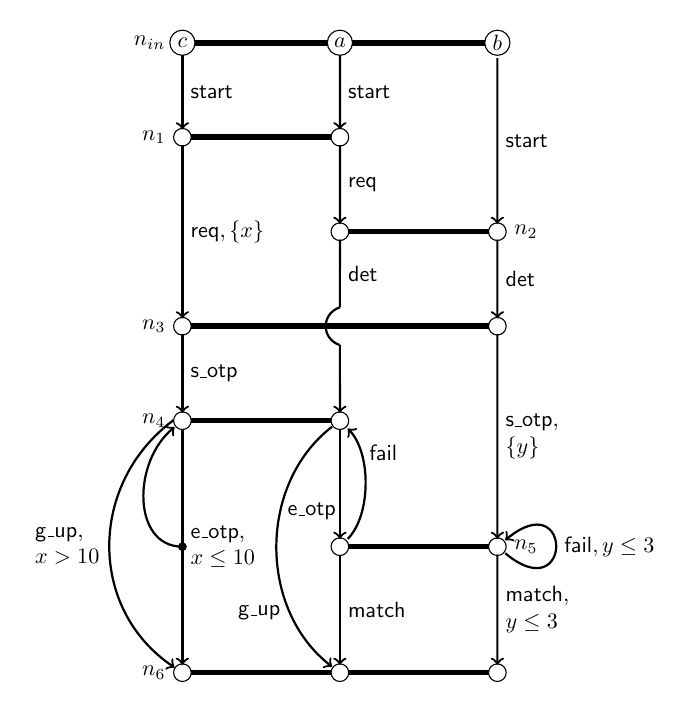
\begin{tikzpicture}[scale=0.8, every node/.style={transform shape}]

\begin{scope}[line width=2pt]
  \draw (0.,0) node [left] {$n_{\text{in}}\,\,$} -- (5,0); 
  \draw (0.,-1.5) node [left] {$n_{1}\,\,$} -- (2.5,-1.5); 
  \draw (2.5,-3) -- (5,-3) node [right] {$\,\,n_{2}$}; 
  \draw (0.,-4.5) node [left] {$n_{3}\,\,$} -- (5,-4.5); 
  \draw (0.,-6) node [left] {$n_{4}\,\,$} -- (2.5,-6); 
  \draw (2.5,-8) -- (5,-8) node [right] {\,\,$n_{5}$}; 
  \draw (0.,-10) node [left] {$n_{6}\,\,$} -- (5,-10);
\end{scope}

\begin{scope}[fill=white]
  \filldraw (0,0) circle (2mm) node (nic) {$c$}; 
  \filldraw (2.5,0) circle (2mm) node (nia) {$a$}; 
  \filldraw (5,0) circle (2mm) node (nib) {$b$};

  \filldraw (0,-1.5) circle (1.4mm) node (n1c) {}; 
  \filldraw (2.5,-1.5) circle (1.4mm) node (n1a) {};

  \filldraw (2.5,-3) circle (1.4mm) node (n2a) {}; 
  \filldraw (5,-3) circle (1.4mm) node (n2b) {};

  \filldraw (0,-4.5) circle (1.4mm) node (n3c) {}; 
  \filldraw (5,-4.5) circle (1.4mm) node (n3b) {};

  \filldraw (0,-6) circle (1.4mm) node (n4c) {}; 
  \filldraw (2.5,-6) circle (1.4mm) node (n4a) {};

  \filldraw (2.5,-8) circle (1.4mm) node (n5a) {}; 
  \filldraw (5,-8) circle (1.4mm) node (n5b) {};

  \filldraw (0,-10) circle (1.4mm) node (n6c) {}; 
  \filldraw (2.5,-10) circle (1.4mm) node (n6a) {}; 
  \filldraw (5,-10) circle (1.4mm) node (n6b) {};

  \filldraw [fill=black] (0,-8) circle (0.6mm) node (v1) {};
\end{scope}

\begin{scope}[thick,->]
  \draw (nic) -- (n1c) node [right, midway] {$\mathsf{start}$}; 
  \draw (n1c) -- (n3c) node [right, midway] {$\mathsf{req}, \{x\}$}; 
  \draw (n3c) -- (n4c) node [right, midway] {$\mathsf{s\_otp}$}; 
  \draw (n4c) -- (n6c) node [right, text width = 1.2 cm, midway] {$\mathsf{e\_otp},$ $x\leq10$}; 
  \draw (0,-8) .. controls (-0.8,-8) and (-0.8,-6.65) .. (n4c);

  \draw (nia) -- (n1a) node [right, midway] {$\mathsf{start}$}; 
  \draw (n1a) -- (n2a) node [right, midway] {$\mathsf{req}$}; 
  \draw (2.5,-4.8) -- (n4a); 
  \draw (n4a) -- (n5a) node [left=-0.3cm, text width = 1 cm, near end] {$\mathsf{e\_otp}$}; 
  \draw (n5a) -- (n6a) node [right, text width = 1 cm, midway] {$\mathsf{match}$}; 
  \draw (n5a) .. controls (3,-7.5) and (3,-6.5) .. (n4a) node [right, near end] {$\mathsf{fail}$}; 
  \draw (n4a) .. controls (1.2,-7) and (1.2,-9) .. (n6a) node [left=-0.3cm, text width = 1 cm, near end] {$\mathsf{g\_up}$};

  \draw (nib) -- (n2b) node [right, midway] {$\mathsf{start}$}; 
  \draw (n2b) -- (n3b) node [right, midway] {$\mathsf{det}$}; 
  \draw (n3b) -- (n5b) node [right, text width = 1 cm, midway] {$\mathsf{s\_otp},$ $\{y\}$}; 
  \draw (n5b) -- (n6b) node [right, text width = 1 cm, midway] {$\mathsf{match},$ $y\leq3$}; 
  \draw (n5b) .. controls (6.2,-9) and (6.2,-7) .. (n5b) node [right, midway] {$\mathsf{fail}, y\leq3$};

  \draw (n4c) + (-0.14,0.01) .. controls (-1.5,-7) and (-1.5,-9) .. (n6c) node [left=-0.2cm, text width = 1.25 cm, midway] {$\mathsf{g\_up},$ $x > 10$};
\end{scope}

\draw [thick] (n2a) -- (2.5,-4.2) node [right, midway] {$\mathsf{det}$}; 
\draw [thick] (2.5,-4.2) .. controls (2.2,-4.3) and (2.2,-4.7) .. (2.5,-4.8);
\end{tikzpicture}
\caption{ATM transaction as a local-timed negotiation. Customer $c$ has local clock $x$ (reset at $\mathsf{req}$, checked at $\mathsf{e\_otp}$ and $\mathsf{g\_up}$). Bank $b$ has local clock $y$ (reset at $\mathsf{s\_otp}$, checked at $\mathsf{match}$ and $\mathsf{fail}$). Annotations like "$x \leq 10$" are guards; "$\{x\}$" indicates clock reset.}
\label{fig:ATM}
\end{figure}

\paragraph{Agent local clocks.} Each agent maintains local clocks:
\begin{itemize}
\item Customer $c$ has clock $x$ and reference clock $t_c$,
\item ATM $a$ has reference clock $t_a$ (no additional local clocks in this example),
\item Bank $b$ has clock $y$ and reference clock $t_b$.
\end{itemize}

Reference clocks $t_c, t_a, t_b$ measure each agent's total elapsed time. They are never reset and never appear in guards—they serve only to track local time progression. Regular clocks like $x$ and $y$ can be reset and used in guards to express timing constraints.

\paragraph{How timing constraints work.} Consider the customer's 10-unit deadline:
\begin{enumerate}
\item At outcome $\mathsf{req}$ (node $n_1$), customer $c$ resets clock $x$ to zero. This marks the start of their personal timer.
\item Time elapses locally: $c$ experiences some delay before $n_3$ (OTP receipt), then more delay before $n_4$ (OTP entry).
\item At outcome $\mathsf{e\_otp}$ (from $n_4$), the guard $x \leq 10$ is checked. This outcome is enabled only if $c$'s local clock $x$ hasn't exceeded 10 units.
\item If $x > 10$, the alternative outcome $\mathsf{g\_up}$ (give up) becomes the only option, with guard $x > 10$.
\end{enumerate}

Similarly, the bank's 3-unit security window:
\begin{enumerate}
\item At outcome $\mathsf{s\_otp}$ (node $n_3$), bank $b$ resets clock $y$ to zero, starting the OTP validity timer.
\item Validation at $n_5$ checks $y \leq 3$ for both $\mathsf{match}$ and $\mathsf{fail}$ outcomes, ensuring validation attempts occur within the window.
\end{enumerate}

\paragraph{Local time progression.} Between interactions, agents' reference clocks can advance by different amounts. For instance:
\begin{itemize}
\item Customer $c$ might hesitate for 2 units before entering the OTP ($t_c$ advances by 2),
\item Meanwhile, bank $b$ might experience only 0.5 units of processing time ($t_b$ advances by 0.5),
\item ATM $a$ might wait 1.8 units for network communication ($t_a$ advances by 1.8).
\end{itemize}

This reflects the asynchronous reality of distributed systems. Regular clocks like $x$ and $y$ evolve with their agent's reference clock: if $t_c$ advances by 2 units, so does $x$ (unless reset).

\paragraph{Illustrative run.}
We briefly illustrate the semantics using the ATM example of
Figure~\ref{fig:ATM}.  Consider the initial configuration $(C_0,v_0)$, where
$C_0(p)=\{n_{in}\}$ for all agents and all clocks are $0$.

Suppose the customer $c$ delays by $4$ time units, the bank $b$ by $1$ unit, and
the ATM $a$ by $0$ units.  This corresponds to the delay vector
$\Delta(c)=4$, $\Delta(b)=1$, $\Delta(a)=0$, yielding a valuation $v_1$ with
$v_1(t_c)=4$, $v_1(t_b)=1$, and $v_1(t_a)=0$.  All local clocks of an agent advance
together with its reference clock.

At this point, the outcome $st$ at the initial node can be executed provided that
all guards are satisfied.  If the initial node is synchronizing, then in addition
we must have $v_1(t_c)=v_1(t_b)=v_1(t_a)$; otherwise the action is blocked, and a
different delay vector must be chosen.  After executing the action, the marking
is updated according to the outcome, and the specified local clocks are reset.

This example illustrates two characteristic features of the semantics: delay
choices are made independently by agents, but synchronization may retroactively
restrict which delay vectors are admissible, and resets affect only local clocks,
never the reference clocks.

\paragraph{Why this matters.} The local-time semantics captures realistic timing behavior that global-time models cannot express naturally:
\begin{itemize}
\item Each agent enforces its own deadlines independently,
\item Timing constraints relate events within an agent's experience (e.g., "10 units after I started"),
\item Agents need not progress in lock-step—they coordinate only at interaction points.
\end{itemize}

\subsection{Preview: Synchronization}

The ATM example uses only local clocks and guards—no explicit synchronization of reference clocks. However, some scenarios require temporal alignment. Imagine the bank wants to ensure the customer and ATM begin validation simultaneously (perhaps for two-factor authentication). We could make node $n_5$ a \emph{synchronizing node}, requiring $t_a = t_b$ when $n_5$ occurs.

Sections~\ref{subsec:ltn-causal} and \ref{subsec:ltn-nonregular} explore how synchronization enables powerful modeling patterns—and contributes to undecidability.

%---------------------------------------------------------------------------------

\section{Formal Definition}
\label{sec:ltn-def}

We now formalize local-timed negotiations, building on the control-flow framework from Chapter~\ref{chap:preliminaries}.

\paragraph{Notation.} For a finite set $S$, write $\mathcal{P}(S)$ for its power set (subsets). Let $\mathbb{R}_{\geq 0}$ denote non-negative reals and $\mathbb{N}$ the natural numbers.

\paragraph{Guards.} Let $X$ be a finite set of clocks. A \emph{guard} over $X$ is a conjunction of constraints of the form $x \bowtie c$ where $x \in X$, $\bowtie \in \{<, \leq, =, \geq, >\}$, and $c \in \mathbb{N}$. Write $\Phi(X)$ for the set of guards over $X$. A valuation $v : X \to \mathbb{R}_{\geq 0}$ \emph{satisfies} guard $g$, written $v \models g$, if all constraints in $g$ evaluate to true under $v$.

\begin{definition}[Local-timed negotiation]
\label{def:ltn}
Let $P$ be a finite set of \emph{agents}, $\Sigma$ a finite set of \emph{outcomes}, and $X$ a finite set of \emph{local clocks} partitioned as $X = \bigcup_{p \in P} X_p$ where $X_p$ are the local clocks of agent $p$.

Additionally, each agent $p$ has a distinguished \emph{reference clock} $t_p$. Reference clocks are never reset and never appear in guards. Let $T := \{t_p \mid p \in P\}$ denote the set of all reference clocks.

A \textsf{local-timed negotiation} (LTN) is a tuple:
\[
\mathcal{N} = (N, \text{dom}, \delta, \text{Sync})
\]
where:
\begin{itemize}
\item $N$ is a finite set of \emph{nodes} (atomic negotiations) with a distinguished \emph{initial node} $n_{\text{in}} \in N$,

\item $\text{dom} : N \to \mathcal{P}(P) \setminus \{\emptyset\}$ maps each node to its non-empty set of participating agents (its \emph{domain}), with $\text{dom}(n_{\text{in}}) = P$. For each agent $p \in P$, define $N_p := \{n \in N \mid p \in \text{dom}(n)\}$ as the set of nodes involving $p$.

\item $\delta = \{\delta_p\}_{p \in P}$ is a family of local transition functions, where:
\[
\delta_p : N_p \times \Sigma \to \Phi(X_p) \times \mathcal{P}(N_p) \times \mathcal{P}(X_p).
\]
For a location $(n, a)$ with $p \in \text{dom}(n)$, the value $\delta_p(n, a) = (g_p, M_p, Y_p)$ specifies:
\begin{itemize}
\item $g_p \in \Phi(X_p)$: a \emph{guard} over $p$'s local clocks,
\item $M_p \subseteq N_p$: the set of nodes $p$ becomes ready for after outcome $a$,
\item $Y_p \subseteq X_p$: the set of $p$'s local clocks to reset when outcome $a$ occurs.
\end{itemize}
We call pairs $(n, a)$ \emph{locations}.

\item $\text{Sync} \subseteq N$ is the set of \emph{synchronizing nodes}. At synchronizing nodes, participating agents' reference clocks must be equal.
\end{itemize}
\end{definition}

\paragraph{Intuition recap.} An LTN extends untimed negotiations (Definition~\ref{def:negotiation}) by adding:
\begin{enumerate}
\item \textbf{Local clocks} $X_p$ for each agent to track time within their local frame,
\item \textbf{Reference clocks} $t_p$ to measure total local elapsed time (implicit, never manipulated directly),
\item \textbf{Guards} constraining when outcomes can occur based on local clock values,
\item \textbf{Resets} allowing clocks to be zeroed at interaction points,
\item \textbf{Synchronizing nodes} where temporal alignment (equality of reference clocks) is required.
\end{enumerate}

%---------------------------------------------------------------------------------

\section{Semantics}
\label{sec:ltn-semantics}

The semantics of an LTN describes how the system evolves through delays (time passage) and actions (outcome occurrences). Configurations track both control state (markings) and timing (valuations).

\subsection{Markings, Valuations, and Configurations}

\begin{definition}[Marking]
A \textsf{marking} is a function $C : P \to \mathcal{P}(N)$ where $C(p) \subseteq N_p$ for each agent $p$. The set $C(p)$ records which nodes agent $p$ is currently ready to participate in.
\end{definition}

The initial marking $C_0$ has $C_0(p) = \{n_{\text{in}}\}$ for all $p \in P$.

\begin{definition}[Valuation and well-formedness]
A \textsf{valuation} is a function $v : X \cup T \to \mathbb{R}_{\geq 0}$ assigning real values to all local clocks and reference clocks. A valuation $v$ is \textsf{well-formed} if for every agent $p \in P$ and every local clock $x \in X_p$:
\[
v(x) \leq v(t_p).
\]
\end{definition}

The intuition for well-formedness is that, since local clocks $x \in X_p$ evolve with reference clock $t_p$ and can only be reset to zero (never increased independently), we always have $v(x) \leq v(t_p)$. This invariant ensures clocks don't "run ahead" of local time.

\begin{definition}[Configuration]
A \textsf{configuration} is a pair $(C, v)$ where $C$ is a marking and $v$ is a well-formed valuation. The \textsf{initial configuration} is $(C_0, v_0)$ where $C_0(p) = \{n_{\text{in}}\}$ for all $p$ and $v_0$ maps all clocks in $X \cup T$ to zero.
\end{definition}

\subsection{Transitions: Delays and Actions}

\paragraph{Local delays.} A \emph{local delay vector} is a function $\Delta : P \to \mathbb{R}_{\geq 0}$ assigning each agent a non-negative delay. Given valuation $v$ and local delay $\Delta$, define $v + \Delta$ by:
\[
(v + \Delta)(z) = v(z) + \Delta(p) \quad \text{for all } p \in P \text{ and all } z \in X_p \cup \{t_p\}.
\]

Thus, all clocks belonging to agent $p$ (both local clocks in $X_p$ and reference clock $t_p$) advance together by $\Delta(p)$. Different agents may experience different delays.

\paragraph{Clock resets.} For a set $Y \subseteq X$ of local clocks, write $v[Y \mapsto 0]$ for the valuation that resets clocks in $Y$ to zero and leaves all other clocks unchanged:
\[
v[Y \mapsto 0](z) = \begin{cases}
0 & \text{if } z \in Y, \\
v(z) & \text{otherwise}.
\end{cases}
\]

\paragraph{Delay steps.}
\begin{definition}[Delay step]
A delay step has the form:
\[
(C, v) \xrightarrow{\Delta} (C, v + \Delta)
\]
where $\Delta$ is a local delay vector and $v + \Delta$ is well-formed. The marking is unchanged; only clock values increase.
\end{definition}

\paragraph{Action steps.}
\begin{definition}[Action step]
\label{def:action-step}
Let $(n, a)$ be a location. We write $(C, v) \xrightarrow{(n,a)} (C', v')$ if the following conditions hold:

\begin{enumerate}
\item \textbf{Enablement:} $n \in C(p)$ for all $p \in \text{dom}(n)$. \\
(All participating agents are ready at $n$.)

\item \textbf{Synchronization (if required):} If $n \in \text{Sync}$, then $v(t_p) = v(t_q)$ for all $p, q \in \text{dom}(n)$. \\
(At synchronizing nodes, reference clocks must be equal.)

\item \textbf{Local guards:} For each $p \in \text{dom}(n)$, let $\delta_p(n, a) = (g_p, M_p, Y_p)$. Then $v \models g_p$ for all $p \in \text{dom}(n)$. \\
(All local guards are satisfied.)

\item \textbf{Marking update:} Define $C'$ by:
\[
C'(p) = \begin{cases}
M_p & \text{if } p \in \text{dom}(n) \text{ and } \delta_p(n,a) = (g_p, M_p, Y_p), \\
C(p) & \text{if } p \notin \text{dom}(n).
\end{cases}
\]
(Participating agents update readiness; others remain unchanged.)

\item \textbf{Clock resets:} Let $Y = \bigcup_{p \in \text{dom}(n)} Y_p$ where $\delta_p(n,a) = (g_p, M_p, Y_p)$ for $p \in \text{dom}(n)$. Then $v' = v[Y \mapsto 0]$. \\
(All clocks in reset sets are zeroed; reference clocks never reset.)
\end{enumerate}
\end{definition}

\paragraph{Small steps and runs.}
\begin{definition}[Small step]
A \textsf{small step} combines a delay followed immediately by an action:
\[
(C, v) \xrightarrow{\Delta} (C, v + \Delta) \xrightarrow{(n,a)} (C', v').
\]
Conceptually, agents accumulate delays until the desired location becomes enabled and all guards are satisfied.
\end{definition}

\begin{definition}[Run]
A \textsf{run} is a finite or infinite sequence of small steps starting from the initial configuration $(C_0, v_0)$:
\[
(C_0, v_0) \xrightarrow{\Delta_0} (C_0, v_0 + \Delta_0) \xrightarrow{(n_0, a_0)} (C_1, v_1) \xrightarrow{\Delta_1} \cdots
\]
\end{definition}

\subsection{Location Reachability}

\begin{definition}[Location reachability]
\label{def:location-reachability}
A location $(n, a)$ is \textsf{reachable} if there exists a run that executes it. The \textsf{location-reachability problem} asks: given an LTN $\mathcal{N}$ and a location $(n, a)$, does there exist a run executing $(n, a)$?
\end{definition}

This is the central decision problem studied in this thesis. As we'll see, unrestricted LTNs have undecidable location reachability.

\paragraph{Untimed projection.} The \emph{untimed outcome language} of $\mathcal{N}$ is the set of words $w = a_0 a_1 \cdots a_k \in \Sigma^*$ for which there exists a run whose executed locations are $(n_0, a_0), (n_1, a_1), \ldots, (n_k, a_k)$. This abstracts away delays, retaining only the sequence of outcomes.

\begin{figure}[t]
\centering
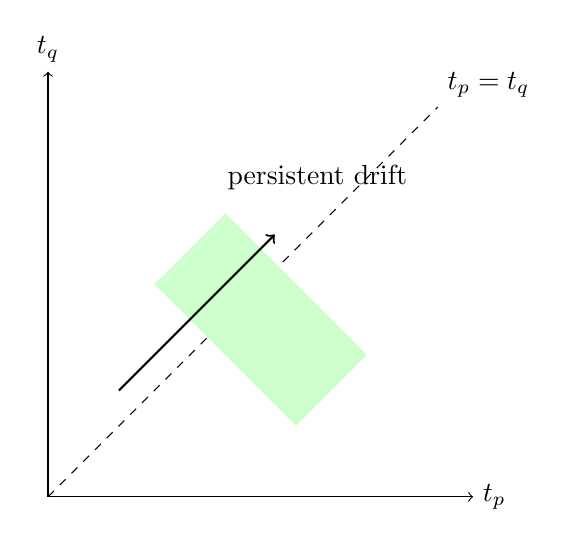
\begin{tikzpicture}[scale=0.9]

% Axes
\draw[->] (0,0) -- (6,0) node[right] {$t_p$};
\draw[->] (0,0) -- (0,6) node[above] {$t_q$};

% Diagonal
\draw[dashed] (0,0) -- (5.5,5.5) node[above right] {$t_p = t_q$};

% Drift region
\fill[green!20] (1.5,3) -- (2.5,4) -- (4.5,2) -- (3.5,1) -- cycle;

% Trajectory
\draw[thick,->] (1,1.5) -- (2,2.5) -- (3.2,3.7);

% Label
\node at (3.8,4.5) {persistent drift};

\end{tikzpicture}
\caption{Independent local time evolution allows relative timing differences
between agents to persist across interactions.}
\label{fig:persistent-drift}
\end{figure}

%---------------------------------------------------------------------------------

\subsection{Design choices and modelling rationale}
\label{subsec:ltn-design}

Local-timed negotiations combine ideas from negotiations and timed automata, but
the resulting model reflects a number of deliberate design choices.  We briefly
discuss the most important ones and contrast them with plausible alternatives.

\paragraph{Local clocks and delay vectors.}
Time elapse in LTNs is described by delay vectors $\Delta \in \Rpos^{P}$, rather
than by a single global delay.  This reflects the intended local-time semantics:
each agent progresses according to its own clock, and different agents may
accumulate time at different rates.  Using a single delay, as in timed automata,
would collapse the model back to a global-time view and eliminate the possibility
of drift between agents.

\paragraph{Reference clocks.}
Each agent $p$ is equipped with a reference clock $t_p$ that is never reset and
never appears in guards.  Reference clocks serve as a semantic device for tracking
the accumulated local time of an agent across the execution.  By excluding
reference clocks from guards, we ensure that agents cannot directly observe or
test global time; instead, comparisons between reference clocks are possible only
indirectly, via explicit synchronization.

\paragraph{Synchronization as a constraint.}
In LTNs, synchronization is expressed as the equality constraint
$t_p = t_q$ at synchronizing nodes, rather than as an instantaneous time jump or
reset.  Equality must be achieved by choosing appropriate local delays before the
action.  This makes synchronization an explicit modelling choice and separates
``time passing'' from ``time comparison'' in the semantics.

\paragraph{Node-based synchronization.}
Synchronization is associated with nodes (atomic negotiations) rather than with
outcomes.  This aligns with the interaction-centric nature of negotiations: timing
constraints are imposed at the level of joint interactions, not at the level of
local control-flow choices.

\paragraph{Local guards and resets.}
Guards and resets are local to each participating agent.  This prevents implicit
global coordination through shared clocks and ensures that all cross-agent timing
dependencies arise either from the negotiation structure itself or from explicit
synchronization nodes.

%---------------------------------------------------------------------------------

\section{Expressiveness}
\label{sec:ltn-expressiveness}

Here we understand the model better via two more examples.

\subsection{Causal Enforcement Through Synchronization}
\label{subsec:ltn-causal}

In global-time models, causality arises from control flow and shared clocks. LTNs add a new mechanism: \emph{using synchronization to force intermediate interactions}. An agent can be compelled to perform actions (accumulate local time) to align with a partner's reference clock.

\begin{example}[Forcing intermediate interactions via timing]
\label{ex:vendor}
Consider three agents: $p$, $q$, and a vendor $v$. Agent $p$ wants to ensure that $q$ has visited the vendor between their two meetings. Figure~\ref{fig:vendor} shows how this can be enforced using local clocks and synchronization.

\begin{figure}[t]
\centering
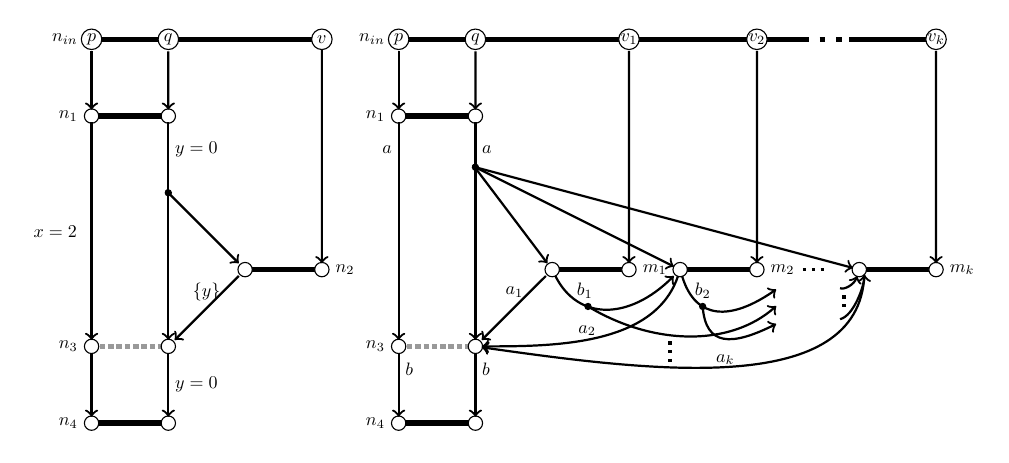
\begin{tikzpicture}[scale=0.65, every node/.style={transform shape}]

\begin{scope}[shift={(-6,0)}]
\begin{scope}[line width=2pt]
\draw (0.,0) node [left] {$n_{in}\,\,$} -- (4.5,0);
\draw (0,-1.5) node [black, left, opacity=1] {$n_1\,\,$} -- (1.5,-1.5);
\draw (3,-4.5)  -- (4.5,-4.5) node [right] {\,\,$n_2$};
\draw [densely dotted, opacity=0.4] (0,-6) node [black, left, opacity=1] {$n_3\,\,$} -- (1.5,-6);
\draw (0,-7.5) node [left] {$n_{4}\,\,$} -- (1.5,-7.5);
\end{scope}

\filldraw [fill=white]  (0,0)  circle (2mm) node 		(nip) {$p$};
\filldraw [fill=white]  (1.5,0)  circle (2mm) node 		(niq) {$q$};
\filldraw [fill=white]  (4.5,0)  circle (2mm) node 		(niv) {$v$};

\filldraw [fill=white]  (0,-1.5)  circle (1.4mm) node 	(n1p) {};
\filldraw [fill=white]  (1.5,-1.5)  circle (1.4mm) node (n1q) {};

\filldraw [fill=black]  (1.5,-3) circle (.6mm) node		(virt) {};

\filldraw [fill=white]  (3,-4.5)  circle (1.4mm) node 	(n21) {};
\filldraw [fill=white]  (4.5,-4.5)  circle (1.4mm) node (n2v) {};

\filldraw [fill=white]  (0,-6)  circle (1.4mm) node 	(n3p) {};
\filldraw [fill=white]  (1.5,-6)  circle (1.4mm) node 	(n3q) {};

\filldraw [fill=white]  (0,-7.5)  circle (1.4mm) node 	(nfp) {};
\filldraw [fill=white]  (1.5,-7.5)  circle (1.4mm) node (nfq) {};


\begin{scope}[thick,->]

\draw (nip) -- (n1p);
\draw (n1p) -- (n3p) node [midway, left, text width = 1cm] {$x=2$};
\draw (n3p) -- (nfp) node [midway, left] {};

\draw (niq) -- (n1q);
\draw (n1q) -- (n3q) node [very near start, right] {$y=0$};
\draw (virt) + (-.05,.05) -- (n21);
\draw (n21) -- (n3q) node [midway, above] {$\{y\}$};
\draw (n3q) -- (nfq) node [midway, right, text width = 1cm] {$y=0$};

\draw (niv) -- (n2v);

\end{scope}
\end{scope}

\begin{scope}[line width=2pt]
\draw (0.,0) node [left] {$n_{in}\,\,$} -- (7.9,0);
\draw (8.8,0) node [left] {} -- (10.5,0);
\draw (0,-1.5) node [black, left, opacity=1] {$n_1\,\,$} -- (1.5,-1.5);
\draw (3,-4.5)  -- (4.5,-4.5) node [right] {\,\,$m_1$};
\draw (5.5,-4.5)  -- (7,-4.5) node [right] {\,\,$m_2$};
\draw (9,-4.5)  -- (10.5,-4.5) node [right] {\,\,$m_k$};
\draw [densely dotted, opacity=0.4] (0,-6) node [black, left, opacity=1] {$n_3\,\,$} -- (1.5,-6);
\draw (0,-7.5) node [left] {$n_{4}\,\,$} -- (1.5,-7.5);
\end{scope}

\filldraw [fill=white]  (0,0)  circle (2mm) node 		(nip) {$p$};
\filldraw [fill=white]  (1.5,0)  circle (2mm) node 		(niq) {$q$};
\filldraw [fill=white]  (4.5,0)  circle (2mm) node 		(niv) {$v_1$};
\filldraw [fill=white]  (7,0)  circle (2mm) node 		(niv2) {$v_2$};
\filldraw [fill=white]  (10.5,0)  circle (2mm) node 		(nivk) {$v_k$};

\filldraw [fill=white]  (0,-1.5)  circle (1.4mm) node 	(n1p) {};
\filldraw [fill=white]  (1.5,-1.5)  circle (1.4mm) node (n1q) {};

\filldraw [fill=black]  (1.5,-2.5) circle (.6mm) node		(virt) {};

\filldraw [fill=white]  (3,-4.5)  circle (1.4mm) node 	(n21) {};
\filldraw [fill=white]  (4.5,-4.5)  circle (1.4mm) node (n2v) {};

\filldraw [fill=white]  (0,-6)  circle (1.4mm) node 	(n3p) {};
\filldraw [fill=white]  (1.5,-6)  circle (1.4mm) node 	(n3q) {};

\filldraw [fill=white]  (0,-7.5)  circle (1.4mm) node 	(nfp) {};
\filldraw [fill=white]  (1.5,-7.5)  circle (1.4mm) node (nfq) {};

\filldraw [fill=white]  (5.5,-4.5)  circle (1.4mm) node 	(v2q) {};
\filldraw [fill=white]  (7,-4.5)  circle (1.4mm) node (v2v) {};

\filldraw [white, fill=white]  (7.5,-4.8)  circle (1.4mm) node (virt2) {};
\filldraw [white, fill=white]  (8.5,-4.8)  circle (1.4mm) node (virt3) {};
\filldraw [white, fill=white]  (8.5,-5.5)  circle (1.4mm) node (virt8) {};

\filldraw [fill=black]  (3.7,-5.22)  circle (.6mm) node (virt4) {};
\filldraw [fill=black]  (5.94,-5.22)  circle (.6mm) node (virt5) {};

\filldraw [white, fill=white]  (7.5,-5.1)  circle (1.4mm) node (virt6) {};
\filldraw [white, fill=white]  (7.5,-5.5)  circle (1.4mm) node (virt7) {};

\filldraw [fill=white]  (9,-4.5)  circle (1.4mm) node 	(vkq) {};
\filldraw [fill=white]  (10.5,-4.5)  circle (1.4mm) node (vkv) {};

\begin{scope}[thick,->]

\draw (nip) -- (n1p);
\draw (n1p) -- (n3p) node [very near start, left] {$a$};
\draw (n3p) -- (nfp) node [near start, right, text width = 1cm] {$b$};

\draw (niq) -- (n1q);
\draw (n1q) -- (n3q) node [very near start, right] {$a$};
\draw (virt) + (-.05,.05) -- (n21);
\draw (n3q) -- (nfq) node [near start, right, text width = 1cm] {$b$};

\draw (niv) -- (n2v);

\draw (niv2) -- (v2v);
\draw (nivk) -- (vkv);

\draw (1.5,-2.5) -- (v2q);
\draw (1.5,-2.5) -- (vkq);

\draw (n21) -- (n3q) node [near start, left = 0cm] {$a_1$};

\end{scope}

\draw [line width=2pt, loosely dotted] (7.9,0)  -- (8.8,0) {};
\draw [very thick, dotted] (7.9,-4.5)  -- (8.4,-4.5) {};
\draw [very thick, dotted] (8.7,-5)  -- (8.7,-5.3) {};
\draw [very thick, dotted] (5.3,-5.9)  -- (5.3,-6.3) {};

\draw [thick,->] (n21) .. controls (3.5,-5.5) and(4.5,-5.5) .. (v2q) node [very near start, right = 0.1cm] {$b_1$};
\draw [thick,->] (v2q) .. controls (5.8,-5.5) and(6.5,-5.5) .. (virt2) node [very near start, right = 0cm] {$b_2$};
\draw [thick,->] (virt3) .. controls (8.7,-4.9) and (8.9,-4.8) .. (vkq);
\draw [thick,->] (virt8) .. controls (8.9,-5.4) and (9.1,-4.8) .. (9.1,-4.6);
\draw [thick,->] (v2q) .. controls (5,-6) and (3,-6) .. (n3q) node [midway, above left= -0.1cm] {$a_2$};
\draw [thick,->] (3.7,-5.22) .. controls (5,-6) and (6.5,-6) .. (virt6);
\draw [thick,->] (5.94,-5.22) .. controls (6,-6) and (6.5,-6) .. (virt7);
\draw [thick,->] (9.1,-4.6) .. controls (9,-7) and (5,-6.5) .. (n3q) node [midway, above left = -0.1cm] {$a_k$};;

\end{tikzpicture}
\caption{Vendor enforcement example. Nodes $n_1$ and $n_3$ are synchronizing (shown with dotted style). At $n_1$, outcome $a$ has guards $x = 2$ for $p$ and $y = 0$ for $q$. At $n_3$, outcome $b$ requires $y = 0$ for $q$. Synchronization forces $q$ to visit vendor $v$ at $n_2$ to accumulate the needed 2 time units. In the figure on the right, the $a$ transition has guards $x = m$ for $p$ and $y = 0$ for $q$. Each $b_i$ transition has a guard $y=1$ and a reset of $y$ to ensure exactly $1$ unit of time is spent in the nodes $m_i$ before outcomes $b_i$. The outcomes $a_i$ have a reset of $y$. The $b$ transition from $n_3$ has a guard $y=0$.}   
	\label{fig:vendor}
\end{figure}

\paragraph{Setup.} Agents $p$ and $q$ have local clocks $x$ and $y$ respectively. Nodes $n_1$ and $n_3$ are synchronizing. At $n_1$, outcome $a$ has guard $x = 2$ for $p$ and $y = 0$ for $q$.

\paragraph{What happens.} After outcome $a$ at $n_1$:
\begin{itemize}
\item Agent $p$ has advanced its reference clock by exactly 2 units (enforced by guard $x = 2$), so $t_p = 2$.
\item Agent $q$ has not advanced at all (guard $y = 0$), so $t_q = 0$.
\end{itemize}

Now both agents are ready at $n_3$ (control-flow wise), and $n_3$ is synchronizing. For outcome $b$ to occur at $n_3$:
\begin{itemize}
\item Synchronization requires $t_p = t_q$, but currently $t_p = 2$ and $t_q = 0$.
\item The guard at $b$ requires $y = 0$ for agent $q$. Since $y$ evolves with $t_q$, letting time elapse for $q$ would make $y > 0$, violating the guard.
\end{itemize}

\paragraph{The only solution.} Agent $q$ cannot simply wait—doing so would violate the guard $y = 0$. Instead, $q$ must:
\begin{enumerate}
\item Visit node $n_2$ (interaction with vendor $v$),
\item Spend exactly 2 time units there (advancing $t_q$ by 2),
\item Reset clock $y$ to zero when leaving $n_2$,
\item Return to $n_3$ with $t_q = 2$ and $y = 0$, satisfying both synchronization and the guard.
\end{enumerate}

This demonstrates \emph{causal enforcement}: the structure of timing constraints and synchronization forces $q$ to take a specific path through the negotiation. Agent $p$ can compel $q$ to perform intermediate interactions by setting up a timing mismatch that can only be resolved by those interactions.
\end{example}

\paragraph{Generalization.} This pattern extends to forcing $q$ to visit $m$ out of $k$ vendors, each requiring $1$ time unit. By setting $p$ delay to $m$ at $n_1$ and requiring $q$ to accumulate exactly $m$ time units before resynchronizing at $n_3$, we force $q$ to interact with at least $m$ vendors. This shows that LTNs can encode counting and comparison—foreshadowing undecidability.

\paragraph{Contrast with global time.} In networks of timed automata with global time, all clocks advance uniformly. One cannot create a situation where agent $p$ is "ahead" of agent $q$ in a way that forces $q$ to perform compensating actions. The local-time semantics is essential for this expressiveness.

\subsection{Non-Regular Untimed Languages}
\label{subsec:ltn-nonregular}

A fundamental result for timed automata is that their untimed languages (projecting runs onto actions, ignoring delays) are always regular. This reflects the finite-state nature of the control structure. Remarkably, LTNs can generate non-regular untimed languages.

\begin{example}[Generating $\{a^n b^n c^n \mid n \geq 0\}$]
\label{ex:anbn}
Consider the LTN in Figure~\ref{fig:abc} with two agents $p$ and $q$. Agent $p$ performs action $a$ repeatedly at node $n_1$, and agent $q$ performs action $b$ repeatedly at node $n_2$. Both can then synchronize at node $n_3$ to perform action $c$.

\begin{figure}[htb]
\centering
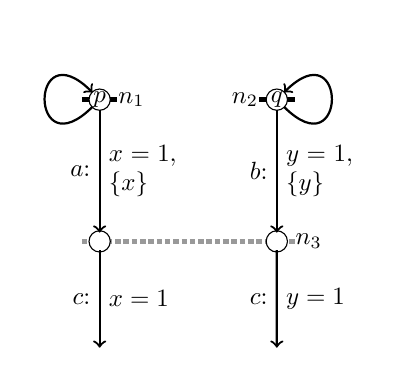
\begin{tikzpicture}[scale=0.9, every node/.style={transform shape}]

\begin{scope}[line width=2pt]
\draw (-.25,0) -- (0.25,0);
\draw (2.25,0) -- (2.75,0);
\draw [opacity=0.4, densely dotted] (-.25,-2) -- (2.75,-2);
\end{scope}

\filldraw [fill=white] (0,0) circle (1.5mm) node (pa) {$p$};
\filldraw [fill=white] (2.5,0) circle (1.5mm) node (qb) {$q$};
\filldraw [fill=white] (0,-2) circle (1.5mm) node (pc) {};
\filldraw [fill=white] (2.5,-2) circle (1.5mm) node (qc) {};

\node at (0.45,0) {$n_1$};
\node at (2.05,0) {$n_2$};
\node at (2.95,-2) {$n_3$};

\begin{scope}[thick,->]
\draw (pa) + (0,-.14) -- (pc) node [midway, left] {$a$:} node [midway, right, text width=1cm] {$x=1,$ $\{x\}$};
\draw (qb) + (0,-.14) -- (qc) node [midway, left] {$b$:} node [midway, right, text width = 1cm] {$y=1,$ $\{y\}$};
\draw (pc) -- (0,-3.5) node [midway, left] {$c$:} node [midway, right, text width=1cm] {$x=1$};
\draw (qc) -- (2.5,-3.5) node [midway, left] {$c$:} node [midway, right, text width=1cm] {$y=1$};
\draw (-0.1,-0.1) .. controls (-1,-1) and (-1,1) .. (-0.1,0.1);
\draw (2.6,-0.1) .. controls (3.5,-1) and (3.5,1) .. (2.6,0.1);
\end{scope}

\end{tikzpicture}
\caption{Non-regular untimed language. Each loop iteration of $a$ and $b$ takes exactly 1 time unit. Node $n_3$ is synchronizing with guards $x = 1$ and $y = 1$. This forces the number of $a$s to equal the number of $b$s before $c$ occurs.}
\label{fig:abc}
\end{figure}

\paragraph{Mechanism.} Both $p$ and $q$ start with reference clocks at zero. Each iteration of $a$ at $n_1$ takes exactly 1 time unit (guard $x = 1$, then reset $x$), advancing $t_p$ by 1. Similarly, each $b$ at $n_2$ advances $t_q$ by 1. The loops are concurrent—there's no ordering between $a$s and $b$s.

Node $n_3$ is synchronizing and requires:
\begin{itemize}
\item $t_p = t_q$ (synchronization condition),
\item $x = 1$ and $y = 1$ (guards at outcome $c$).
\end{itemize}

For these conditions to hold simultaneously:
\begin{itemize}
\item Both agents must have performed their last loop iteration exactly 1 time unit ago,
\item Both agents must have performed the same number of loop iterations (so $t_p = t_q$).
\end{itemize}

Therefore, if $p$ performs $n$ iterations of $a$ and $q$ performs $m$ iterations of $b$, action $c$ can occur if and only if $n = m$. The untimed language includes all words of the form $w \cdot c$ where $w$ has equal number of $a$ and $b$. Note that we can add another identical process with identical guards and which also time-synchronizes at $n_3$, and then the language would be beyond context-free.
\end{example}

\paragraph{Why this matters.} This demonstrates that:
\begin{enumerate}
\item LTNs can encode \emph{counting} constraints across concurrent actions,
\item Synchronization acts as a \emph{comparison} operator between accumulated counts (via reference clocks),
\item The untimed behavior transcends finite-state structure—language-theoretically, LTNs are more powerful than timed automata.
\end{enumerate}

\begin{table}[t]
\centering
\begin{tabular}{ll}
\hline
\textbf{Feature} & \textbf{Enables} \\
\hline
Local delays & Independent progress and drift \\
Reference clocks & Persistent timing information across interactions \\
Synchronizing nodes & Comparison of accumulated drift \\
Unsynchronized nodes & Unbounded drift accumulation \\
Guards and resets & Counter-style encodings via timing constraints \\
\hline
\end{tabular}
\caption{Sources of expressiveness in local-timed negotiations.}
\label{tab:ltn-expressiveness}
\end{table}

This expressiveness enables rich modelling but also implies undecidability, as we'll see next.

%---------------------------------------------------------------------------------
\begin{figure}[t]
\centering
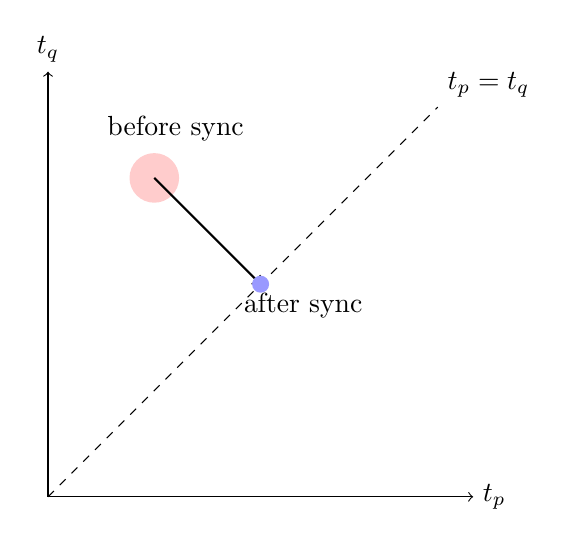
\begin{tikzpicture}[scale=0.9]

% Axes
\draw[->] (0,0) -- (6,0) node[right] {$t_p$};
\draw[->] (0,0) -- (0,6) node[above] {$t_q$};

% Diagonal
\draw[dashed] (0,0) -- (5.5,5.5) node[above right] {$t_p = t_q$};

% Pre-synchronization region
\fill[red!20] (1.5,4.5) circle (0.35);
\node at (1.8,5.2) {before sync};

% Arrow to diagonal
\draw[thick,->] (1.5,4.5) -- (3,3);

% Post-synchronization point
\fill[blue!40] (3,3) circle (0.12);
\node at (3.6,2.7) {after sync};

\end{tikzpicture}
\caption{A time-synchronizing interaction collapses relative timing differences,
allowing accumulated information to be compared or reset.}
\label{fig:selective-sync}
\end{figure}

\section{Undecidability of reachability}
\label{sec:ltn-undec}

\paragraph{Proof roadmap.}
The undecidability proof proceeds by a reduction from the halting problem of
$2$-counter machines.  The key idea is to encode counter values as differences
between reference clocks of carefully chosen agents.

Increment and decrement operations are implemented by allowing certain agents to
accumulate local time while others are forced to remain idle.  Zero-tests rely on
synchronizing nodes, which require equality of reference clocks and thus permit
the comparison of accumulated drift.  Unsynchronized nodes are essential for
allowing drift to grow without bound, while synchronized nodes are essential for
testing and transferring this information.

The construction alternates systematically between synchronized and
unsynchronized phases.  This interplay is what enables the simulation of
unbounded counters and ultimately yields undecidability of
location-reachability.

We now show that location-reachability for LTNs is undecidable.  The proof reduces
the halting problem of $2$-counter machines to reachability in an LTN.  The key
source of power is the unbounded drift between reference clocks of different agents,
together with the ability to impose synchronization at selected nodes.

\begin{theorem}
\label{thm:undecidability}
Location-reachability is undecidable for local-timed negotiations.
\end{theorem}

The rest of the section is devoted to proving
Theorem~\ref{thm:undecidability}. We will encode the halting problem
of a $2$-counter machine as the reachability problem for a local-timed
negotiation.

\subsection{Two-counter machines}
\label{subsec:2cm}

\noindent \emph{Counter machines.} A $2$-counter machine $M$ is a program that manipulates two counters, $C_1$ and $C_2$,
each of which can hold a non-negative number. The machine is given as
a sequence of labelled instructions $\ell:I$, where $I$ is one of the following for some $i \in \{1, 2\}$: 
\begin{description}
\item[increment] $C_i + +$, which increments the value of the
  counter $C_i$ and goes to the next instruction
  $\ell+1$.
\item[decrement] if $C_i>0$ then $C_i- -$, which decrements $C_i$ and continues with the next instruction
  $\ell+1$. If the value of $C_i$ is $0$, then the program is blocked. 
\item[jump-on-zero] if $C_i= = 0$ goto $\ell'$, which transfers control to the instruction labelled $\ell'$ if counter $C_i$ is $0$ for
  $i\in\{1,2\}$. If $C_i>0$, it continues to the instruction $\ell+1$.
\end{description}
The counter machine is said to halt if it reaches the final
instruction. A configuration of $M$ is a triple $(\ell, c_1, c_2)$ representing the current instruction $\ell$ that needs to be executed and the current values $c_1, c_2 \ge 0$ of the counters $C_1, C_2$ respectively. The transitions $(\ell, c_1, c_2) \xra{} (\ell', c'_1, c'_2)$ follow naturally from the description above.

\subsection{Overview of the reduction}
\label{subsec:red-overview}

The negotiation $\Nn_M$ that we
construct will have $6$ agents $p_1, q_1, r_1, p_2, q_2, r_2$. Agents
$p_1, q_1, r_1$ simulate counter $C_1$, and the rest simulate
$C_2$. Let $i \in \{1, 2\}$. The local clocks of $p_i, q_i, r_i$ are
respectively $\{x_{p_i}\}$, $\{x_{q_i}, x'_{q_i}\}$ and $\{x_{r_i}\}$. Additionally, we have the reference clocks $t_\a$ for each agent $\a$. For every instruction $\ell$, we will have a node
$n_\ell$ in which all the six agents participate.
A configuration $(C, v)$ of $\Nn_M$ is said to encode configuration
$(\ell, c_1, c_2)$ of $M$ if:
\begin{itemize}
\item $C(\a) = \{n_\ell\}$ for every agent $\a$,
\item $v(x) = 0$ for all local clocks (and reference clocks can take any value),
\item $v(t_{r_1}) \le v(t_{q_1}) \le v(t_{p_1})$ and $v(t_{r_2}) \le v(t_{q_2}) \le v(t_{p_2})$, and 
\item $v(t_{p_1} - t_{q_1}) = c_1$ and $v(t_{p_2} - t_{q_2}) = c_2$,
\end{itemize}
The initial configuration of $\Nn_M$ has every agent in $n_{\ell_0}$, where $\ell_0$ is the first instruction in $M$ and every clock (including reference clocks) to be $0$. Since reference clocks are never reset and only increase through delay
steps, differences between reference clocks are preserved unless
explicitly modified by controlled delay.

We will have a gadget in $\Nn_M$ corresponding to each instruction in the counter machine. Let $(C, v), (C',v')$ be configurations that encode $(\ell, c_1, c_2)$ and $(\ell', c'_1, c'_2)$ respectively. A run $(C, v) \xra{} \cdots \xra{} (C', v')$ such that none of the intermediate configurations encodes any counter machine configuration will be called a \emph{big step}. We denote a big step as $(C, v) \Rightarrow (C', v')$. Our gadgets will ensure the following two properties.
\begin{itemize}
\item Let $(\ell, c_1, c_2) \xra{} (\ell', c'_1, c'_2)$ in $M$. Then from every configuration $(C, v)$ that encodes $(\ell, c_1, c_2)$, there is a big step $(C, v) \Rightarrow (C', v')$ to some configuration $(C', v')$ that encodes $(\ell', c'_1, c'_2)$.
\item Let $(C, v), (C', v')$ be arbitrary configurations of $\Nn_M$ that encode $(\ell, c_1, c_2)$ and $(\ell', c'_1, c'_2)$ respectively. If $(C, v) \Rightarrow (C', v')$ is a big step, then $(\ell, c_1, c_2) \xra{} (\ell', c'_1, c'_2)$ in $M$.
\end{itemize}
The first property ensures that for every path $(\ell^0, c^0_1, c^0_2)
\xra{} (\ell^1, c^1_1, c^1_2) \xra{} \cdots$, there is a sequence of
big steps $(C_0, v_0) \Rightarrow (C_1, v_1) \Rightarrow \cdots$ such
that  $(C_i, v_i)$ encodes $(\ell^i, c^i_1, c^i_2)$. The second
property ensures the reverse: from a sequence of big steps, we get
a corresponding run in counter machine. We will now describe each
gadget and show that the two properties are satisfied.  

Throughout the gadgets, guards of the form $x=0$ ensure that no agent can
let time elapse before executing the corresponding action; any positive
delay would violate the guard and block the run.

\subsection{Instruction gadgets}
\label{subsec:gadgets}

\begin{figure}[t]
\begin{center}
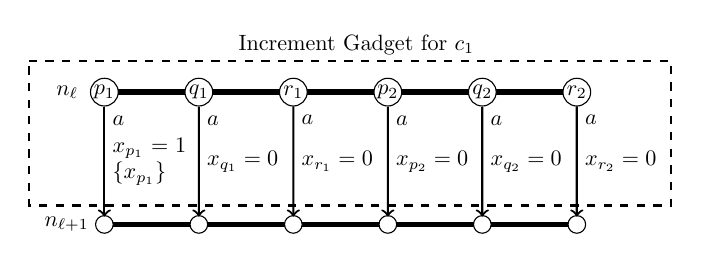
\begin{tikzpicture}[scale=0.8, every node/.style={transform shape}]

\begin{scope}[line width=2pt]
\draw (0,0) -- (7.5,0);
\draw (0,-2.1) -- (7.5,-2.1);
\end{scope}

\filldraw [fill=white]  (0,0)	  circle (2.2mm) node (nip1) [label={left:$n_{\ell}$}] {$p_1$};
\filldraw [fill=white]  (1.5,0)	  circle (2.2mm) node (niq1) {$q_1$};
\filldraw [fill=white]  (3,0)	  circle (2.2mm) node (nir1) {$r_1$};
\filldraw [fill=white]  (4.5,0)	  circle (2.2mm) node (nip2) {$p_2$};
\filldraw [fill=white]  (6,0)	  circle (2.2mm) node (niq2) {$q_2$};
\filldraw [fill=white]  (7.5,0)	  circle (2.2mm) node (nir2) {$r_2$};
\filldraw [fill=white]  (0,-2.1)	  circle (1.4mm) node (n2p1) [label={left:$n_{\ell + 1}$}] {};
\filldraw [fill=white]  (1.5,-2.1)	  circle (1.4mm) node (n2q1) {};
\filldraw [fill=white]  (3,-2.1)	  circle (1.4mm) node (n2r1) {};
\filldraw [fill=white]  (4.5,-2.1)	  circle (1.4mm) node (n2p2) {};
\filldraw [fill=white]  (6,-2.1)	  circle (1.4mm) node (n2q2) {};
\filldraw [fill=white]  (7.5,-2.1)	  circle (1.4mm) node (n2r2) {};

\begin{scope}[thick,->]
  \draw (nip1) -- node [very near start, right] {$a$} (n2p1)	 node [midway,right, text width=1.25cm] {$x_{p_1}=1$ $\{x_{p_1}\}$};
  \draw (niq1) -- node [very near start, right] {$a$} (n2q1)	 node [midway,right, text width=1.25cm] {$x_{q_1}=0$};
  \draw (nir1) -- node [very near start, right] {$a$} (n2r1)	 node [midway,right, text width=1.25cm] {$x_{r_1}=0$};
  \draw (nip2) -- node [very near start, right] {$a$} (n2p2)	 node [midway,right, text width=1.25cm] {$x_{p_2}=0$};
  \draw (niq2) -- node [very near start, right] {$a$} (n2q2)	 node [midway,right, text width=1.25cm] {$x_{q_2}=0$};
  \draw (nir2) -- node [very near start, right] {$a$} (n2r2)	 node [midway,right, text width=1.25cm] {$x_{r_2}=0$};
\end{scope}

\draw [dashed, thick] (-1.2,0.5) -- (9,0.5) -- (9,-1.8) -- (-1.2,-1.8) -- (-1.2,0.5);

\node at (4,.75) {Increment Gadget for $c_1$};
\end{tikzpicture}
\caption{Gadget for implementing increment instruction on $c_1$}
\label{fig:increment}
\end{center}
\end{figure}


\noindent \emph{Increment.} Assume an instruction $\ell: C_1 ++$ with $\ell$ not being the final instruction. The case with $C_2++$ is symmetric. Every configuration $(\ell, c_1, c_2)$ on executing this instruction goes to $(\ell + 1, c_1 + 1, c_2)$. Figure~\ref{fig:increment} shows the gadget for the increment instruction. All agents other than $p_1$ cannot elapse time due to the guard checking local clocks to $0$. Agent $p_1$ elapses
exactly one time unit, after which clock $x_{p_1}$ is reset.
It is easy to see that the configuration $(C', v')$ that results from $(C, v)$
encodes $(\ell', c_1 + 1, c_2)$. The big step $(C, v) \Rightarrow (C',v')$ is in fact a single transition. Both the properties are easily seen to be satisfied. 

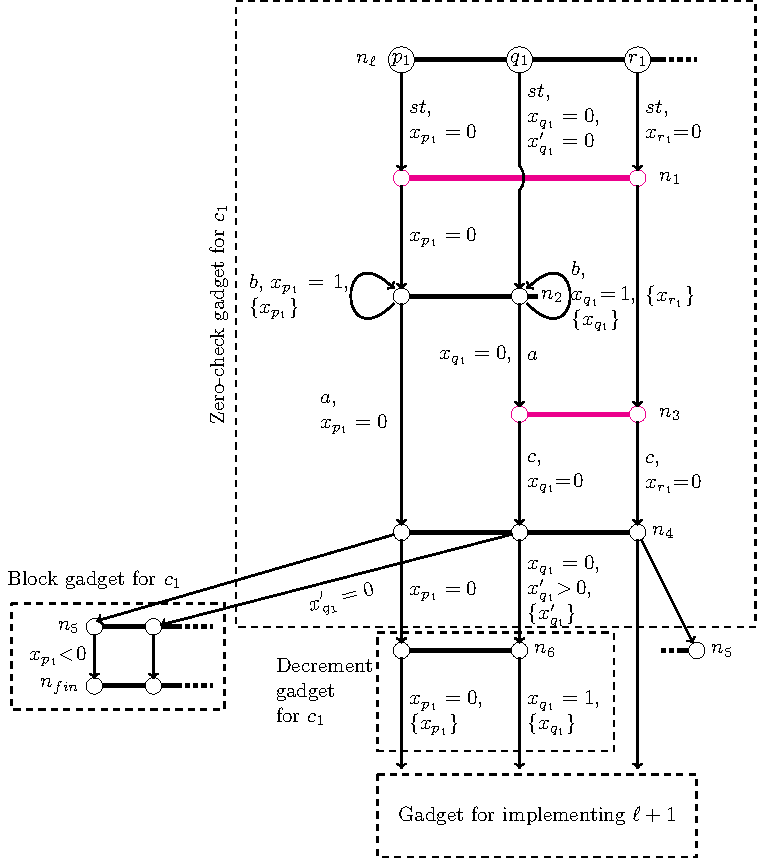
\includegraphics{decrement-gadget.pdf}

\paragraph*{Decrement.} Consider a decrement instruction: if $C_1 > 0$
then $C_1 --$. We have
$(\ell, c_1, c_2) \xra{} (\ell+1, c_1 - 1, c_2)$ if $c_1 > 0$. The
first task is to check if $c_1 > 0$. Recall that in the negotiation the difference $t_{p_1} - t_{q_1}$ gives the value of $c_1$. Our idea is to let $q_1$ elapse time to
synchronize with $p_1$ and check if this time elapse needed for
synchronization is strictly above $0$ or not. However, in this
process, we lose the actual value of the counter. In order to maintain the same difference between $t_{p_1}$ and $t_{q_1}$, we make use of the auxiliary process $r_1$.

Consider a configuration $(C, v)$ that encodes $(\ell, c_1, c_2)$. By our definition, $v(t_{r_1}) \le v(t_{p_1})$ and $v(t_{p_1} - t_{q_1}) = c_1$. 
\begin{itemize}
 
\item We first let $r_1$ synchronize with $p_1$, while $p_1$
  elapses no time.
\item Next, we keep moving both $p_1$ and $q_1$ by $1$ unit each until
  $q_1$ synchronizes with $r_1$. In this entire process $r_1$ is not
  allowed to elapse time.
\end{itemize}
By the end of this, we will get a valuation $v'$ with the same difference $v'(t_{p_1} - t_{q_1}) = c_1$
since both the agents were moved by the same amount. Moreover, we can
use an additional clock to check whether in the process of $q_1$
synchronizing with $r_1$, a non-zero time had elapsed in $q_1$.

The gadget is depicted in Figure~\ref{fig:jump-decrement}. For simplicity, we do not index the intermediate nodes $n_1, n_2, n_3, n_4$ by $\ell$. The computation proceeds in three phases. Below, we show the run of $\Nn_M$ along this gadget, restricted to the agents $p_1, q_1, r_1$. The other three agents simply move to the next possible instruction (this is not shown in the figure for simplicity). 

\smallskip

\noindent \emph{Phase 1.} Synchronize $r_1$ with $p_1$ maintaining no time
elapse in $p_1$ as follows: $((n_\ell, n_\ell, n_\ell), v) \xra{}
((n_1, n_2, n_1), v_1) \xra{} ((n_2, n_2, n_3), v_3)$. After the last
action, agents $p_1$ and $r_1$ are synchronized, that is,
$v_3(t_{p_1}) = v_3(t_{r_1})$. This is due to the node $n_1$ being a
synchronization node. Moreover, $v_3(t_{p_1}) = v(t_{p_1})$, due to
the guard $x_{p_1} = 0$. Similarly, $v_3(t_{q_1}) = v(t_{q_1})$ due to
$x_{q_1} = 0$.

\smallskip

\noindent \emph{Phase 2.} Move $p_1$ and $q_1$ repeatedly by one unit each:  $((n_2, n_2, n_3), v_3) \xra{b} ((n_2, n_2, n_3), v_3^1) \xra{b} \cdots \xra{b} ((n_2, n_2, n_3), v_3^k)$. By the end of $k$ iterations of $b$, we have $v^k_3(t_{p_1}) = v(t_{p_1}) + k$ and $v^k_3(t_{q_1}) = v(t_{q_1}) + k$.

\smallskip

\noindent \emph{Phase 3.} Check if the reference clocks of $q_1$ and $r_1$
are equal: $((n_2, n_2, n_3), v_3^k)$
$\xra{a} ((n_4, n_3, n_3), v_4) \xra{c} ((n_4, n_4, n_4), v_5)$. The
outcome $c$ at $n_4$ can be fired only if the reference clocks of
$q_1$ and $r_1$ are equal: that is, $v_4(t_{q_1}) = v_4(t_{r_1})$. Due
to the guard checking for $0$ at $a$ and $c$, we have
$v_5(t_{q_1}) = v_4(t_{q_1}) = v_3^k(t_{q_1})$. From Phase 2, this
value equals $v(t_{q_1}) + k$. Secondly, notice that
$v_4(t_{r_1}) = v_3(t_{r_1})$, which from Phase 1 equals
$v(t_{p_1})$. From the equality $v_4(t_{q_1}) = v_4(t_{r_1})$, we get
$v(t_{q_1}) + k = v(t_{p_1})$.  This shows that
$k = v(t_{p_1}) - v({t_{q_1}})$. The number of times the loop $b$ is
done equals the difference between $t_{p_1}$ and $t_{q_1}$ at the
start of this gadget. If the number of $b$ iterations is more than
this value or less than this value, location $(n_3, c)$ cannot be
executed and the negotiation cannot proceed further. At the end of the gadget, the ordering
$v(t_{r_1}) \le v(t_{q_1}) \le v(t_{p_1})$ is restored, ensuring that
subsequent gadgets operate under the same encoding invariant.


When action $c$ is done, the clock $x'_{q_1}$ holds the time between
$st$ and $c$ for agent $q_1$, and this is exactly $k$. If $k > 0$ the
value of $t_{q_1}$ is increased by $1$, resulting in the counter value
getting decremented and the agents move to the next instruction (shown
as the decrement gadget in the figure). Otherwise, the agents are sent
to a gadget from which there is no run (shown as the block gadget in
the figure).
Notice the interplay between synchronized and unsynchronized nodes in
this gadget. It is crucial that $n_2$ is unsynchronized, whereas
nodes $n_1, n_3$ need to be.
Note that after Phase~1 the value of $t_{r_1}$ remains fixed throughout
Phase~2, while each execution of $b$ strictly increases $t_{q_1}$.
Hence, once $t_{q_1} > t_{r_1}$, equality can never be restored, and the
final synchronization test necessarily fails.

%diagram for intuition

\paragraph{Concrete example.}
We illustrate the decrement gadget with a concrete example.  Consider a
configuration $(C,v)$ encoding $(\ell,c_1,c_2)$ with $c_1=2$, so that
$v(t_{p_1}) - v(t_{q_1}) = 2$ and all local clocks are $0$.

\emph{Positive case ($c_1>0$).}
In Phase~1, agent $r_1$ synchronizes with $p_1$ without any time elapse in $p_1$,
so after synchronization we have
$v(t_{r_1}) = v(t_{p_1})$ and still $v(t_{p_1}) - v(t_{q_1}) = 2$.
In Phase~2, the loop labeled $b$ is executed twice, advancing both $p_1$ and
$q_1$ by one unit each time.  After two iterations, $q_1$ reaches the same
reference time as $r_1$, and synchronization at the next node becomes possible.
Since a positive amount of time has elapsed in this phase, the gadget proceeds
to the decrement branch, reducing the encoded counter value from $2$ to $1$.

\emph{Zero case ($c_1=0$).}
Now suppose $(C,v)$ encodes $c_1=0$, so that
$v(t_{p_1}) = v(t_{q_1})$ initially.  Phase~1 again synchronizes $r_1$ with
$p_1$.  In Phase~2, the loop $b$ cannot be executed even once: advancing $q_1$
would immediately make its reference clock larger than that of $r_1$, and the
final synchronization test would fail.  Consequently, no run can reach the
decrement branch, and the execution is forced into the blocking gadget.

This example shows how the feasibility of synchronization distinguishes the
cases $c_1>0$ and $c_1=0$ without directly testing the counter value.

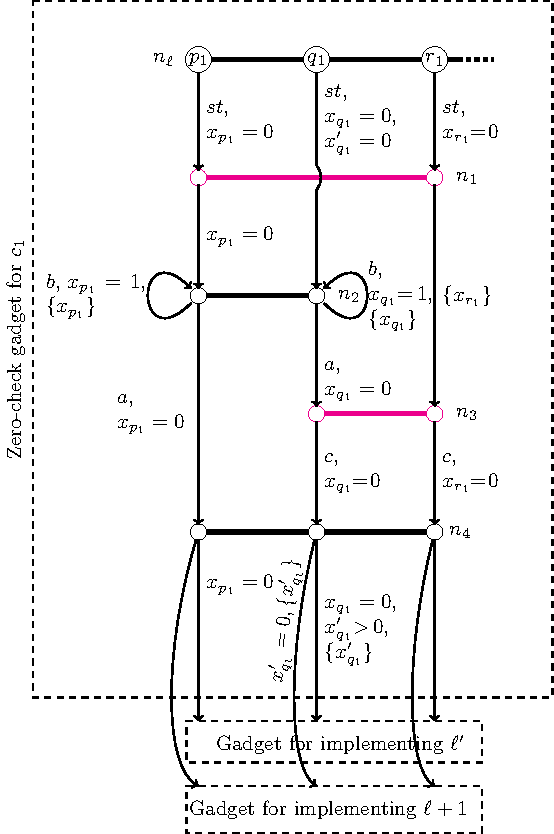
\includegraphics{jump-gadget.pdf}

\noindent \emph{Jump-on-zero.} This gadget is similar to the decrement
gadget, where the first part was to check if $C_1$ is $0$ or not. When $C_1 == 0$, the gadget jumps to the
relevant instruction, otherwise it moves to the next instruction in
sequence. The gadget is shown in~\cite{mukund2023localtime}. 

%---------------------------------------------------------------------------------
\section{Summary and perspective}
\label{sec:summary-ch3}

This chapter introduced \emph{local-timed negotiations} (LTNs) as a real-time
extension of negotiations in which each agent carries its own set of local clocks,
and time elapses \emph{locally} (via delay vectors).  The semantics combines three
ingredients:

\begin{itemize}
  \item the negotiation-style control flow captured by markings (who is ready to
        participate in which node),
  \item local clock constraints (guards and resets attached to outcomes), and
  \item \emph{optional} explicit synchronization at selected nodes, expressed as the
        constraint that all participating agents have equal reference clocks.
\end{itemize}

We illustrated how LTNs model timing constraints between interactions using the
ATM example (Figure~\ref{fig:ATM}).  We then highlighted two expressiveness
phenomena that are characteristic of the local-time setting:
(i) synchronization can be used as a \emph{causal enforcement} mechanism, forcing
agents to perform intermediate interactions (Section~\ref{subsec:ltn-vendor}),
and (ii) the untimed outcome language of an LTN can be non-regular
(Section~\ref{subsec:ltn-nonregular}), in sharp contrast to timed automata where
the untimed language is always regular.

The main algorithmic message of the chapter is negative: we proved that
\emph{location-reachability is undecidable} for LTNs (Theorem~\ref{thm:undecidability})
by a reduction from halting of $2$-counter machines.  Conceptually, the reduction
pinpoints the source of power: reference clocks can drift arbitrarily, and
synchronizing nodes allow the system to \emph{compare} and \emph{transfer}
information encoded in those drifts.  In particular, the proof relies on a careful
interplay between synchronized nodes (where equality of reference clocks must be
met) and unsynchronized nodes (where agents can advance independently and thus
accumulate drift).

\smallskip
\noindent\textbf{Perspective.}
LTNs sit between two well-studied extremes.  On one hand, they inherit the
interaction-centric, partial-order flavour of negotiations; on the other hand,
they adopt a clock-based view of time as in timed automata, but without a global
time line.  This combination is expressive enough to model realistic timing
patterns (local deadlines, response windows, and time-bounded protocols), while
also making plain that \emph{unrestricted} local-time drift together with
\emph{explicit} synchronization yields a model beyond decidability for basic
reachability.

This motivates the rest of the thesis: to identify robust restrictions that
preserve the modelling advantages of LTNs but regain algorithmic tractability.
Two orthogonal axes stand out naturally from this chapter:
\begin{itemize}
  \item restricting (or eliminating) explicit synchronization, so that drift cannot
        be tested directly; and
  \item bounding the amount of drift that can accumulate (globally, per-agent, or
        per-cycle), so that comparisons do not simulate unbounded counters.
\end{itemize}
Understanding where decidability reappears along these axes also clarifies which
expressiveness features (e.g.\ enforcing intermediate interactions, or generating
non-regular untimed languages) survive in the restricted models, and which do not.

\smallskip
\paragraph{What causes undecidability?} The reduction pinpoints two features:
\begin{enumerate}
\item \textbf{Unbounded drift}: Reference clocks can diverge arbitrarily, encoding unbounded integer values (counter contents).
\item \textbf{Explicit synchronization}: Synchronizing nodes allow the system to test equality of reference clocks, enabling comparisons and conditional behavior based on encoded values.
\end{enumerate}

Removing or restricting either feature may recover decidability—this is the focus of Part~II.

%---------------------------------------------------------------------------------
\section{Coming next}
\label{sec:next-ch3}

This chapter concludes Part~I, where we introduced local-timed negotiations and
established that, in their full generality, even basic location-reachability is
undecidable (Theorem~\ref{thm:undecidability}).  The remainder of the thesis
(Part~II) is devoted to recovering decidability by identifying restrictions that
preserve the modelling advantages of LTNs while taming the two sources of
algorithmic hardness exposed by the reduction: \emph{unrestricted drift} between
local reference clocks and the ability to \emph{test} that drift via explicit
synchronization.

Part~II develops several decidable fragments along complementary axes:
\begin{itemize}
  \item \textbf{Extreme synchronization regimes:} we study the two endpoints where
        synchronization is either \emph{forbidden} (synchronization-free LTNs) or
        \emph{mandatory} at every interaction (always-synchronized LTNs), and
        analyze how these extremes change both expressiveness and the reachability
        problem.
  \item \textbf{Quantitative restrictions on drift:} we introduce drift-bounded
        variants that limit how far apart agents' reference clocks may deviate,
        yielding finite (or well-structured) symbolic state spaces.
  \item \textbf{Structural restrictions:} we consider communication/topological
        constraints on the underlying negotiation graph---for instance, connected
        communication patterns---and show how they can re-establish decidability
        even when clocks remain local.
  \item \textbf{Few-process settings:} we isolate the two-process case as a
        particularly informative boundary, where local time still matters but the
        concurrency structure becomes constrained enough to admit specialized
        algorithms.
\end{itemize}

\smallskip
\noindent\textbf{Immediate next chapter.}
We begin Part~II by focusing on the first axis above, namely the two extreme
synchronization regimes: \emph{synchronization-free} LTNs and \emph{always-synchronized}
LTNs.
